\documentclass[11pt]{article} 
\usepackage[english]{babel}
\usepackage[utf8]{inputenc}
\usepackage[margin=0.5in]{geometry}
\usepackage{amsmath}
\usepackage{amsthm}
\usepackage{amsfonts}
\usepackage{amssymb}
\usepackage[usenames,dvipsnames]{xcolor}
\usepackage{graphicx}
\usepackage[colorinlistoftodos, color=orange!50]{todonotes}
\usepackage{hyperref}
\usepackage[numbers, square]{natbib}
\usepackage{fancybox}
\usepackage{epsfig}
\usepackage{soul}
\usepackage[framemethod=tikz]{mdframed}
\usepackage[shortlabels]{enumitem}
\usepackage[version=4]{mhchem}
\usepackage{multicol}
\usepackage{forest}
\usepackage{mathtools}
\usepackage{comment}
\usepackage{enumitem}
\usepackage[utf8]{inputenc}
\usepackage{listings}
\usepackage{color}
\usepackage[numbers]{natbib}
\usepackage{subfiles}
\usepackage{algorithm}
\usepackage[noend]{algpseudocode}


\newtheorem{prop}{Proposition}[section]
\newtheorem{thm}{Theorem}[section]
\newtheorem{lemma}{Lemma}[section]
\newtheorem{cor}{Corollary}[prop]

\theoremstyle{definition}
\newtheorem{definition}{Definition}

\theoremstyle{definition}
\newtheorem{required}{Problem}
\newtheorem*{requiredHC}{Problem HC}

\theoremstyle{definition}
\newtheorem{ex}{Example}

\newcommand{\interval}[4]{\draw (#2, #1) -- (#3, #1); % Usage: \interval{height}{start}{end}{label}
\draw (#2, #1-0.11) -- (#2, #1+0.11); % draw left whisker
\draw (#3, #1-0.11) -- (#3, #1+0.11); % draw right whisker
\node[] at (#2-0.25, #1) {#4};
}


\setlength{\marginparwidth}{3.4cm}
%#########################################################

%To use symbols for footnotes
\renewcommand*{\thefootnote}{\fnsymbol{footnote}}
%To change footnotes back to numbers uncomment the following line
%\renewcommand*{\thefootnote}{\arabic{footnote}}

% Enable this command to adjust line spacing for inline math equations.
% \everymath{\displaystyle}

% _______ _____ _______ _      ______ 
%|__   __|_   _|__   __| |    |  ____|
%   | |    | |    | |  | |    | |__   
%   | |    | |    | |  | |    |  __|  
%   | |   _| |_   | |  | |____| |____ 
%   |_|  |_____|  |_|  |______|______|
%%%%%%%%%%%%%%%%%%%%%%%%%%%%%%%%%%%%%%%

\title{
\normalfont \normalsize 
\textsc{CSCI 3104 Fall 2021 \\ 
Instructors: Profs. Grochow and Waggoner} \\
[10pt] 
\rule{\linewidth}{0.5pt} \\[6pt] 
\huge Problem Set 7 \\
\rule{\linewidth}{2pt}  \\[10pt]
}
%\author{Your Name}
\date{}

\begin{document}
\definecolor {processblue}{cmyk}{0.96,0,0,0}
\maketitle


%%%%%%%%%%%%%%%%%%%%%%%%%
%%%%%%%%%%%%%%%%%%%%%%%%%%
%%%%%%%%%%FILL IN YOUR NAME%%%%%%%
%%%%%%%%%%AND STUDENT ID%%%%%%%%
%%%%%%%%%%%%%%%%%%%%%%%%%%
\noindent
Due Date \dotfill TODO \\
Name \dotfill \textbf{Didi Trifonova} \\
Student ID \dotfill \textbf{109388776} \\
Collaborators \dotfill \textbf{List Your Collaborators Here}

\tableofcontents

\section*{Instructions}
\addcontentsline{toc}{section}{Instructions}
 \begin{itemize}
	\item The solutions \textbf{must be typed}, using proper mathematical notation. We cannot accept hand-written solutions. Useful links and references on \LaTeX can be found \href{https://canvas.colorado.edu/courses/75824/pages/latex}{here on Canvas}.
	\item You should submit your work through the \textbf{class Canvas page} only. Please submit one PDF file, compiled using this \LaTeX \ template.
	\item You may not need a full page for your solutions; pagebreaks are there to help Gradescope automatically find where each problem is. Even if you do not attempt every problem, please submit this document with no fewer pages than the blank template (or Gradescope has issues with it).

	\item You are welcome and encouraged to collaborate with your classmates, as well as consult outside resources. You must \textbf{cite your sources in this document.} \textbf{Copying from any source is an Honor Code violation. Furthermore, all submissions must be in your own words and reflect your understanding of the material.} If there is any confusion about this policy, it is your responsibility to clarify before the due date. 

	\item Posting to \textbf{any} service including, but not limited to Chegg, Reddit, StackExchange, etc., for help on an assignment is a violation of the Honor Code.

	\item You \textbf{must} virtually sign the Honor Code (see Section \hyperlink{HonorCode}{Honor Code}). Failure to do so will result in your assignment not being graded.
\end{itemize}


\section*{Honor Code (Make Sure to Virtually Sign the Honor Pledge)} 
\addcontentsline{toc}{section}{Honor Code (Make Sure to Virtually Sign the Honor Pledge)}
\hypertarget{HonorCode}{}

\begin{requiredHC}
On my honor, my submission reflects the following:
\begin{itemize}
\item My submission is in my own words and reflects my understanding of the material.
\item Any collaborations and external sources have been clearly cited in this document.
\item I have not posted to external services including, but not limited to Chegg, Reddit, StackExchange, etc.
\item I have neither copied nor provided others solutions they can copy.
\end{itemize}

\noindent In the specified region below, clearly indicate that you have upheld the Honor Code. Then type your name. 
\end{requiredHC}

\begin{proof}[(Agreed)]
I agree to the honor code - Didi Trifonova
\end{proof}



\newpage
\section{Standard 19: Tree Method.}

\begin{required}
Consider the recurrence $T(n)$ below. Using the {\bf tree method}, determine a suitable function $f(n)$ such that $T(n) \in \Theta(f(n))$. Clearly show all steps. Note the following:
\begin{itemize}
\item You may assume, without loss of generality, that $n$ is a power of $3$ (i.e., $n = 3^{k}$ for some integer $k \geq 0$).
\item You may hand-draw your tree and embed it, provided it is legible and we do not have to rotate our screens to read it. However, \textbf{all your calculations must be typed}.
\end{itemize}

\[
T(n) = \begin{cases} 1, &  n < 3 \\ 
3T(n/3) + n^{2}, &  \text{otherwise.} \end{cases}
\]

\end{required}

\begin{proof}[Answer] $ $ \\
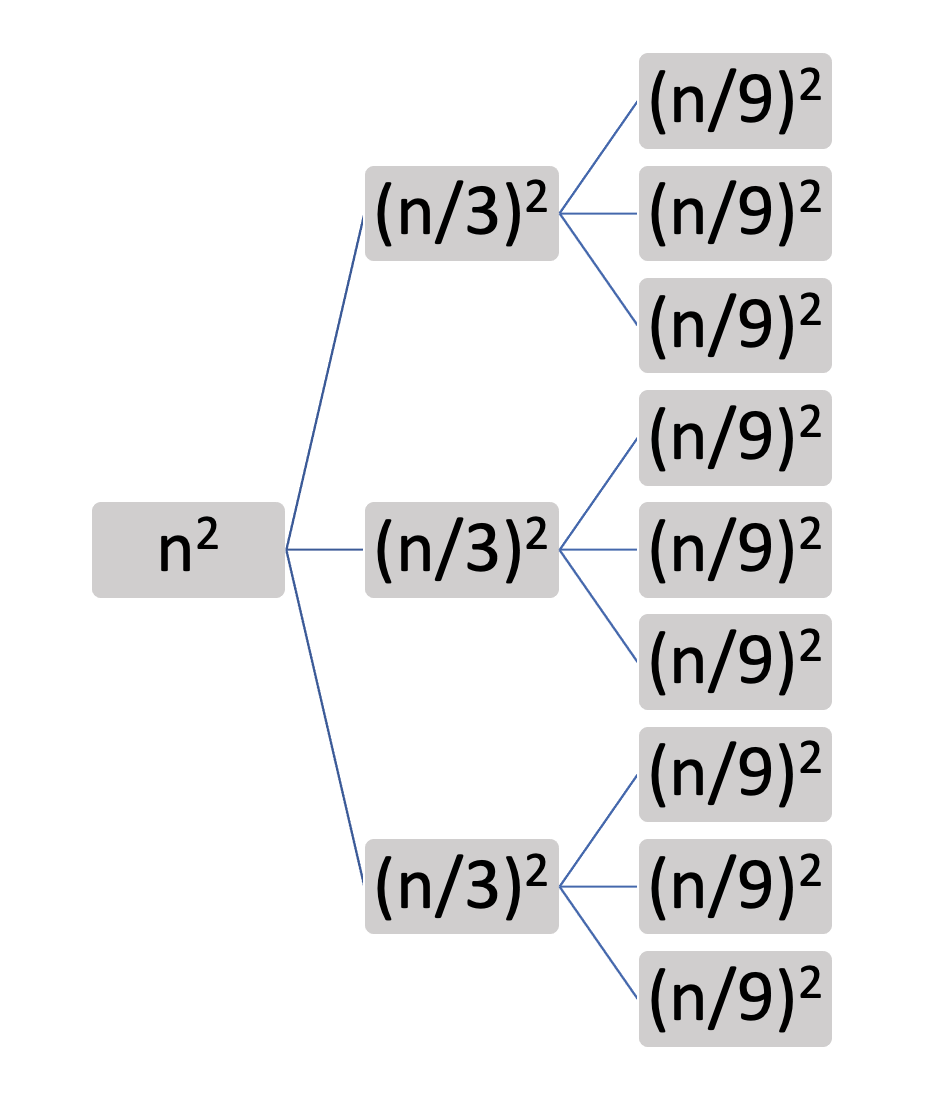
\includegraphics[width=100mm]{prob1.png} \\
\begin{itemize}
    \item level with starting node is $i=0$
    \item A node at level $i$ is equal to $\left( \frac{n}{3^i}\right)^2$ 
    \item The number of nodes at each level is $3^i$
    \item Then, each level is equal to $\frac{n^23^i}{3^{2i}} = \frac{n^2}{3^i}$
    \item This tree will have a total of $log_3n - 1$ levels
\end{itemize}
\begin{align*}
    T(n) &= \sum_{i=0}^{log_3(n)-1} \left( \frac{n^2}{3^i}\right) \\
    &= n^2 \sum_{i=0}^{log_3(n)-1} \left( \frac{1}{3}\right)^i \\
    &= n^2 \left[\frac{1 - (1/3) ^ {log_3n-1+1}}{1-(1/3)}\right] \\
    &= \frac{3n^2}{2}\left[ 1 - (1/3)^{log_3n} \right] \\
    &= \frac{3n^2}{2}\left[ 1 - \frac{1^{log_3n}}{3^{log_3n}} \right] \\
    &= \frac{3n^2}{2}\left[ 1 - \frac{1}{n} \right] \\
    &= \frac{3n^2}{2} - \frac{3}{2} n \\
\end{align*}
$T(n) \in \Theta(n^2)$
\end{proof}



\newpage
\section{Standard 20: Quicksort.}

\begin{required}
\begin{enumerate}[label=(\alph*)]
\subsection{Part \ref{S20a}}

\item \label{S20a} Write down a recurrence relation that models the {\bf best case} running time of Quicksort, i.e. the case where {\sc Partition} selects the {\bf median} element at each iteration.

\begin{proof}[Answer]
% YOUR ANSWER BELOW
\begin{align*}
T(n) = \begin{cases}
\text{$C_1$} & : n \leq 1, \\
\text{$C_2n+2T(\frac{n}{2})$} & : n > 1
\end{cases}
\end{align*}
\end{proof}


\newpage 
\subsection{Part \ref{S20b}}
\item \label{S20b} Write down a recurrence relation that models the {\bf worst case} running time of Quicksort, i.e. the case where {\sc Partition} selects the {\bf last} element at each iteration.

\begin{proof}[Answer]
% YOUR ANSWER BELOW
\begin{align*}
T(n) = \begin{cases}
\text{$C_1$} & : n \leq 1, \\
\text{$C_2n+T(n-1)$} & : n > 1
\end{cases}
\end{align*}
\end{proof}



\newpage
\subsection{Part \ref{S20c} }

\item \label{S20c} Suppose that we modify {\sc Partition}($A,s,e$) so that it chooses the median element of $A[s..e]$ in calls that occur in nodes of even depth of the recursion tree of a call {\sc Quicksort}($A[1, \ldots, n],1, n$), and it chooses the maximum element of $A[s..e]$ in calls that occur in nodes of odd depth of this recursion tree. \\
  
\noindent Assume that the running time of this modified {\sc Partition} is still $\Theta(n)$ on any subarray of length $n$. You may assume that the root of a recursion tree starts at level $0$ (which is an even number), its children are at level 1, etc. \\
  
\noindent \textbf{Your job} is to write down a recurrence relation for the running time of this version of {\sc Quicksort} given an array $n$ distinct elements and solve it asymptotically, i.e.\ give your answer as $\Theta(f(n))$ for some function $f(n)$. Show your work.

\begin{proof}[Answer]
Recurrence relation: 
\begin{itemize}
    \item base case: When $n \leq 1, T(n) = 1$
    \item $T_1(n) = C_2n+2T_2(\frac{n}{2})$ and  $T_2(n) = C_2n+T_1(n-1)$
    \item $T_1(n) = C_2n + 2\left[C_2\left(\frac{n}{2}\right) + T_1 \left(\frac{n}{2} -1\right)\right]$
    % \item $T_1(n) = C_2n + 2\left[C_2\left(\frac{n}{2}\right) + T_1 \left(\frac{n-2}{2}\right)\right]$
    \item $T(n) = C_2n 
    + 2C_2\left(\frac{n}{2}\right) 
    + 2T \left(\frac{n}{2}- 1\right) $
    \item $T(n) = 
     2C_2n
    + 2T \left(\frac{n}{2} - 1\right)$
    \item $T(n) < 2C_2n + 2T(\frac{n}{2})$
\end{itemize}
Using the tree method:  \\
At level $i$, each node is equal to $2C_2(\frac{n}{2^i})$\\
The number of nodes at each level is $2^i$ \\
Thus, each level is equal to $2C_2n$ \\
This tree will have a total of $log_2n$ levels
\end{proof}
\begin{align*}
    T(n) &\leq 2C_2\sum_{i=0}^{log_2(n)} n \\
    &= 2C_2  n \cdot log_2(n)
\end{align*}
Thus, $T(n) \in \Theta (nlog_2(n))$
\end{enumerate}
\end{required}

\end{document} % NOTHING AFTER THIS LINE IS PART OF THE DOCUMENT